The previous chapters gave a deep dive into artifact removal, feature extraction and classification techniques which are widely used in several applications. The methods discussed so far have to be redesigned for a different application leading to researching and experimenting different methods. With the application of Deep learning in BCI, this could be avoided. This chapter focuses on SOTA Deep learning methods that are used in researches and industries. Some architectures can even perform artifact removal, feature extraction and classification all-in-one go. The chapter discusses on different Deep learning techniques classified based on the information it extracts from the signal.

Deep learning approaches are used in several industries and are replacing many existing algorithms as they are inherently adaptive to changes in trends as observed in the data. In BCI, the signal processing methods used are tailored for very specific application or EEG paradigms, EEG signals are exposed to various artifacts that need to be eliminated separately and require expertise in relevant domain for feature engineering. Deep Learning \nomenclature{DL}{Deep Learning} can help researchers to elevate this problem by building representations from input data with or without prior knowledge of ground truth. Deep learning models can be broadly classified as Discriminative, Representative, Generative and Hybrid models. This work focuses on classifying the motor intent of the user online, with a system pre-trained model on data obtained in the same session, hence discriminative models are used. Discriminative models can be further classified into Recurrent Neural Network (RNN) \nomenclature{RNN}{Recurrent Neural Network}and Convolutional Neural Network. These networks are capable of extracting different information from the EEG data which serves as feature vectors. \cite{2020_Survey_DL_BCI} and \cite{2021_Book_Deep_Learning_EEG} provides in-depth survey on methods and applications of various deep learning techniques used in research and industries. 

In \cite{2019_EEG_analysis_DNN}, the authors review more than hundred publications that apply DL to BCI. It reveals that inter subject studies are the most researched, CNNs are the most commonly used approach for EEG signal analysis and most of the publications work on the raw EEG data without any preprocessing. \cite{2021_ML_BCI_review} reviews various advancements and applications of machine learning in BCI. \cite{2020_EEG_WaveletTrans_ANN} developed a single system for diagnosing multiple neurological disorders. DWT were used to separate the EEG signals into sub-bands and then statistical features were extracted from each sub-band, which are then later used in the classifier.

\section{Spatial Information}

Convolutional Neural Networks are very often applied in machine vision systems, used in extracting different spatial features in the image. A typical CNN includes layers such as input layer, convolutional layer, pooling layer, fully connected layer, output layer and activation layer in order. A Batch-norm layer can also be used between the convolution layer and the pooling layer which provides uniformly distributed data and avoids over or undershoot of the activation. Dropout layers are generally used between stacks of above mentioned layers and in the fully connected layer that provides regularization effect to the network and prevents over-fitting. The spatial information is extracted as features using a series or stacks of layers between input and the last pooling layer. Classification is performed in the fully connected layers. 

\cite{2019_MI_CNN_WT} uses Deep Convolutional Neural Networks (DCNN) \nomenclature{DCNN}{Deep Convolutional Neural Network}to classify motor imagery tasks. The raw EEG data is preprocessed to remove any artifacts and time-frequency (TF) \nomenclature{TF}{Time-Frequency} information from the noise-free EEG data is extracted using time-frequency transforms such as STFT and CWT. The TF information is forwarded to a DCNN for further feature extraction and classification. The authors used transfer learning on pre-trained AlexNet to adapt the BCI EEG data. In \cite{2018_BCI_SVM_DNN}, the authors performed motor-imagery EEG signal classification using SVM and DCNN which revealed that data preprocessing for artifact removal influences the classification results drastically. In \cite{2021_MI_DCNN}, it is found that the accuracy of the classification is highest in the very start of the experiment, gradually dropping down to the end of experiment.

\cite{2017_EEG_Wavelet_ANN} developed a Computer Aided Diagnosis(CAD) method to detect Autism spectrum disorder using DWT to decompose EEG signals into approximations and details coefficient for each EEG sub-band, extract statistical features such as mean, variance, skewness, kurtosis and similar features or using Shannon entropy values and, classify using Artificial Neural Network (ANN). The ANN structure used was a simple FCNN with one hidden layer. The study found that using DWT and Shannon entropy achieved better accuracy. 

\cite{2021_Online_EEG_MCNN} proposed a CNN model for a four class EEG MI dataset and compared it to the LDA based classifier. The results showed that CNN performed better in extracting and classifying EEG data. CNN uses the mean of specified numbers of samples as the filter, that slides to get a running average of the EEG data for each channel. 

\cite{2017_1trial_MIEEG_DNN} studied the classification performance on a 2 class data using CNNs and also a conventional signal processing pipeline that uses features such as power, CSP or auto-regression coefficients. The results showed that the CNNs performed better than the conventional signal processing pipeline. The authors proposed a 5-layer CNN model \ref{fig:2017_1trial_MIEEG_DNN_arch} that could observe the spatial and temporal information using a column and row filters in individual layers respectively.

    \begin{figure}[H] 
        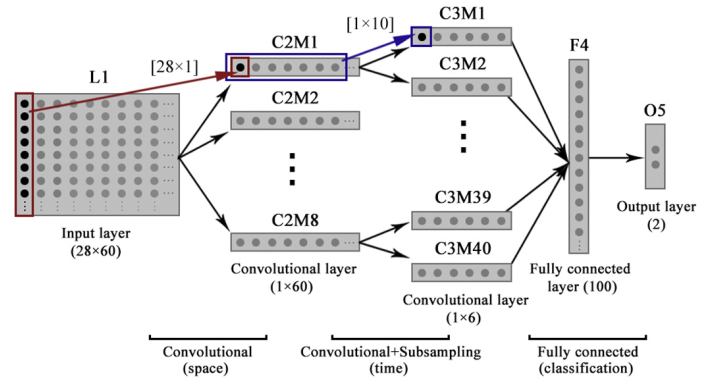
\includegraphics[height=0.6\textwidth]{images/2017_1trial_MIEEG_DNN_arch.png}
        \caption{CNN architecture proposed by \cite{2017_1trial_MIEEG_DNN}(source)}
        \label{fig:2017_1trial_MIEEG_DNN_arch}
    \end{figure}

\cite{2018_EEGNet} designed a single compact CNN architecture that can classify EEG signals from different paradigms using Depthwise and Separable CNNs. The raw EEG signal is convolved with a 1D convolutional filters with a filter length of half of the input sampling rate, resulting in feature maps containing band-passed EEG signal. The spatial information is obtained further using Depthwise convolution, the filters trained in this layer works as a spatial filter. This operation on band-passed EEG signal information enables extraction of frequency specific spatial filters. Finally Separable convolution is applied along with a Pointwise convolution to summarize individual feature maps and optimally combine them. The simple flow diagram given in the figure \ref{fig:eegnet_arch} shows how the depthwise separable convolutions are performed for classification. In this work, this architecture is chosen and implemented for its simplicity and adaptability to different EEG paradigms and experiments.

\begin{figure}[H] 
    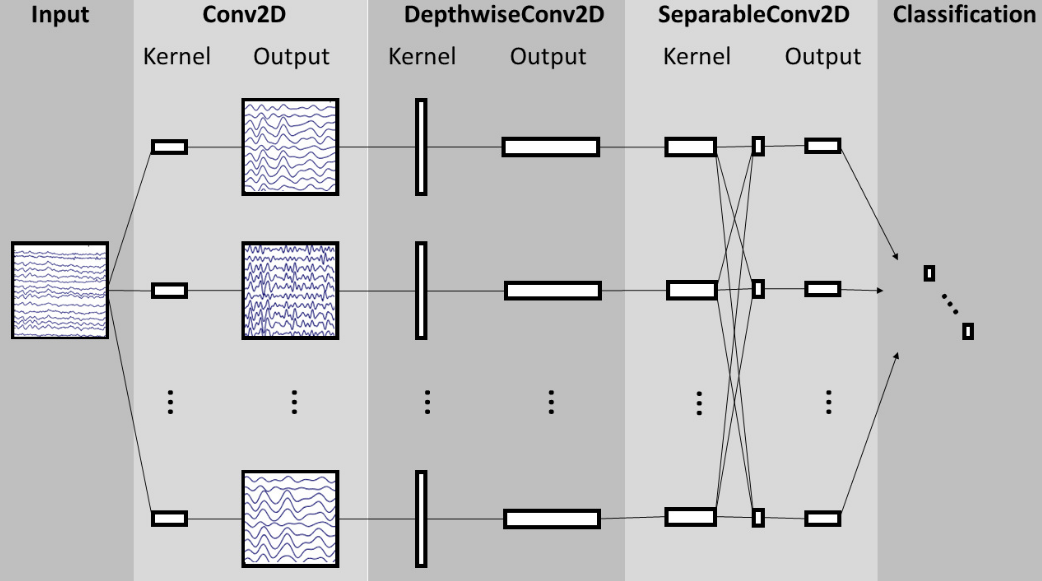
\includegraphics[height=0.6\textwidth]{images/eegnet_arch.png}
    \caption{EEGnet architecture. Source \cite{2018_EEGNet}}
    \label{fig:eegnet_arch}
\end{figure}

\section{Temporal Information}

Recurrent Neural Networks are vastly used in time series applications. They are inherently good at capturing dynamic information in serial data. RNNs have the problem of vanishing or exploding gradients which are overcome by replacing RNN nodes by LSTM cells. LSTM cells have a more complex internal structure that enables to remember data over a long or short time. A typical LSTM cell is shown in figure \ref{fig:lstm_cell}.

    \begin{figure}[H] 
        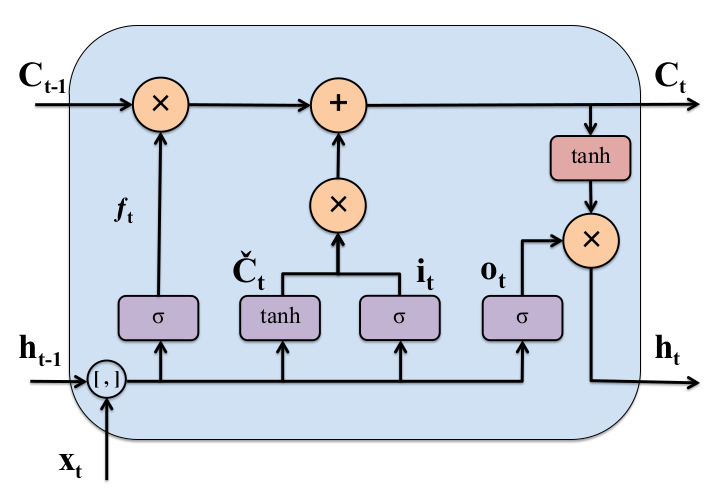
\includegraphics[height=0.6\textwidth]{images/lstm_cell.png}
        \caption{A LSTM cell structure. Source \cite{2018_DL_LSTM}}
        \label{fig:lstm_cell}
    \end{figure}
    
Attention mechanism is generally used at the end of an RNN model to find and weigh importance of each discriminative feature, that assures high classification scores. It is used in Natural Language Processing (NLP) \cite{2018_DL_LSTM} to find the contribution of each word to improve the scores. It amplifies the result by aggregating the hidden states and weighing their relative importance. 

\cite{2019_DLSTM_MI} proposed a solution for classification of hand movements from EEG using a deep attention-based LSTM network by first extracting time and frequency domain features from the EEG signals and passing them to the LSTM input layer. The attention layer captures the importance of the EEG information varying through time where discriminative information with higher importance is assigned higher scores, which results in higher classification results. Time and frequency domain features extracted are listed in \ref{fig:2019_DLSTM_MI_Table2}. The last hidden state of the LSTM is multiplied with trainable weights to capture more discriminative task related features which form the attention mechanism. The network uses 297 features from 7 time steps in each of the 2 second time segment. The entire architecture is given in the figure \ref{fig:2019_DLSTM_MI_arc}. This architecture has been implemented and studied in this thesis.

    \begin{figure}[H] 
    \begin{center}
        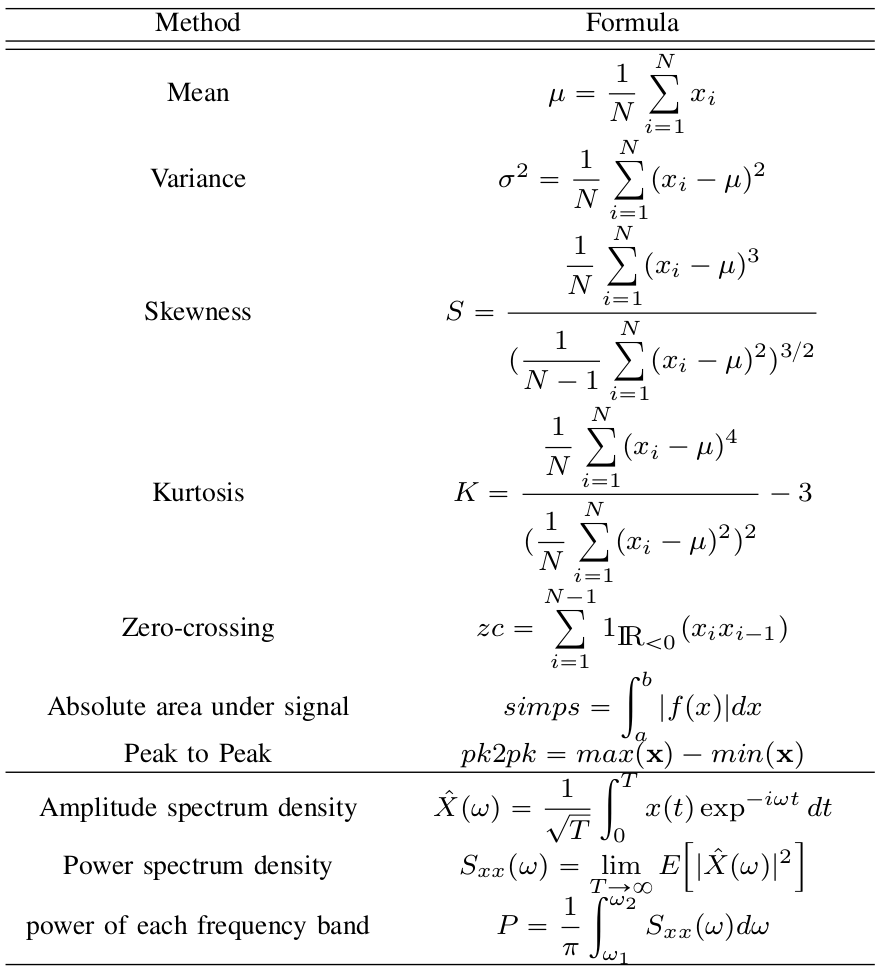
\includegraphics[height=0.6\textwidth]{images/2019_DLSTM_MI_Table2.png}
        \caption{The table of features used by \cite{2019_DLSTM_MI}(source)}
        \label{fig:2019_DLSTM_MI_Table2}
    \end{center}
    \end{figure}

    \begin{figure}[H] 
    \begin{center}
        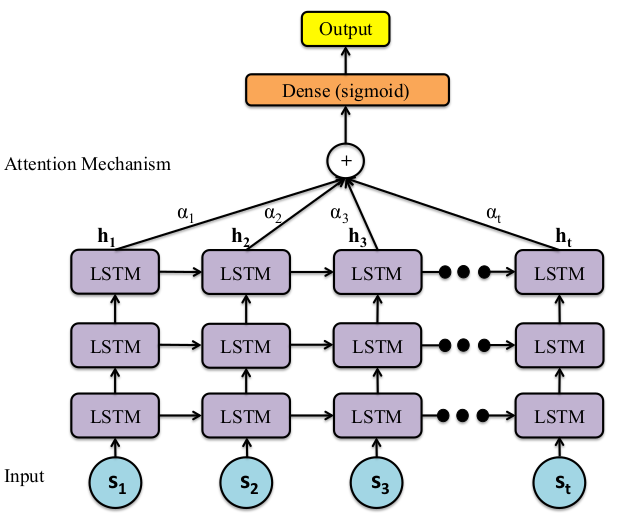
\includegraphics[height=0.6\textwidth]{images/2019_DLSTM_MI_arc.png}
        \caption{A LSTM based architecture proposed by \cite{2019_DLSTM_MI}(source)}
        \label{fig:2019_DLSTM_MI_arc}
    \end{center}    
    \end{figure}

\section{Spatio-Temporal Information}

\cite{2021_DL_LSTM_MI} introduced the cascade and parallel convolutional recurrent neural network to learn the spatio-temporal dynamics of EEG data. The method involves converting 1-dimensional EEG sequences to 2-dimensional EEG meshes, the values of the 2D meshes corresponds to the amplitude from each electrode. At time $t$, the 1D data from all the $n$ electrodes $$r = x_i,  \forall i \in n$$ is converted to 2D mesh with $n$ points and the vacant spaces are set to zero. The 2D meshes are created for each time instance $t$, stacked for a specific time interval $s$ and passed into a cascaded convolutional recurrent neural network \ref{fig:2021_DL_LSTM_MI_CCRNN}. 
    \begin{figure}[H] 
    \begin{center}
        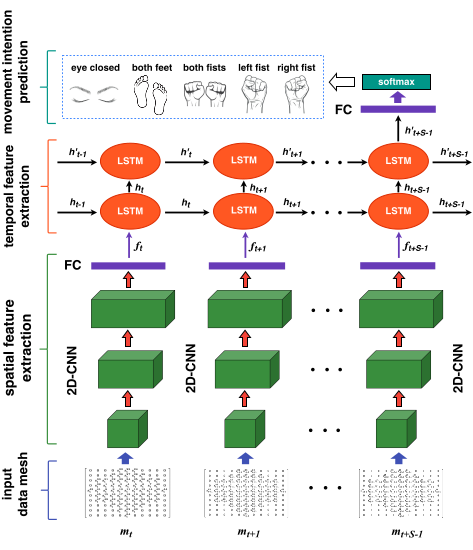
\includegraphics[height=1.0\textwidth]{images/2021_DL_LSTM_MI_CCRNN.png}
        \caption{A Cascaded convolutional recurrent neural network based architecture proposed by \cite{2021_DL_LSTM_MI}(source)}
        \label{fig:2021_DL_LSTM_MI_CCRNN}        
    \end{center}
    \end{figure}

The network first performs spatial feature extraction by a series of $s$ parallel convolution layers followed by a linear layer that fattens the information. The temporal features are extracted from the data by passing the flattened data to the LSTM layers and the output of the last LSTM cell is used to predict the movement intention using softmax as activation layer. \cite{2021_DL_LSTM_MI} also suggests using CNNs and RNNs separately and later concatenate the outputs of the last layers to predict the motor intention of the user using softmax activation layer.

\cite{2021_hDL_BCI} provides  systemic review of several Hybrid Deep Learning models used in BCI research. The study reveals that CNN-RNN hybrid deep learning architectures with Adam optimizer are the most widely researched for extracting spatial-temporal features from the EEG data and the average accuracy is 80 percentage across several datasets. 

\cite{2022_MI_DL_Multilevel} extracts domain-invariant multi-level spatial-temporal features to tackle domain differences. This is done by minimizing the source and target distribution distance.

While the above techniques proposed 2D convolutional neural networks, \cite{2020_DL_LSTM_EEG} proposed 1D CNN-LSTM architecture for automatic recognition of epileptic seizures through EEG signal analysis. Here the EEG data is preprocessed and normalized before the high level spatial information is extracted by the 1D-CNNs and the temporal features by the LSTM layer figure \ref{fig:2020_DL_LSTM_EEG_arch}.

    \begin{figure}[H] 
    \begin{center}
         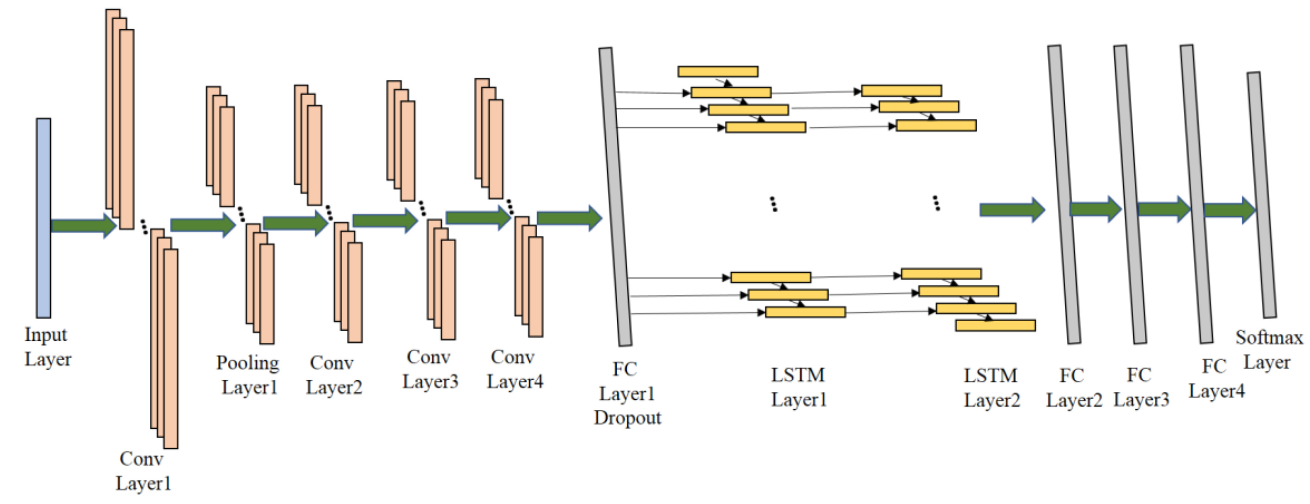
\includegraphics[width=1\textwidth]{images/2020_DL_LSTM_EEG_arch.png}
        \caption{A CNN-LSTM architecture proposed by \cite{2020_DL_LSTM_EEG}(source)}
        \label{fig:2020_DL_LSTM_EEG_arch}       
    \end{center}
    \end{figure}
    
\section{Summary}
Deep Learning is widely been used in BCI systems and researches. Several architectures are developed for a more specific task or problem in BCI. However only few architecture claim adaptability to different BCI applications. Many architectures are discussed above did not require manual removal of artifacts, as they were parameterized and learnt during the process of training. These systems however require retraining and calibration to work for different users and different hardware configurations. In the next chapter, all the implemented algorithms are compared using different datasets on various basis.